\begin{figure}[p]
\centering
    \begin{subfigure}[t]{0.45\textwidth}
    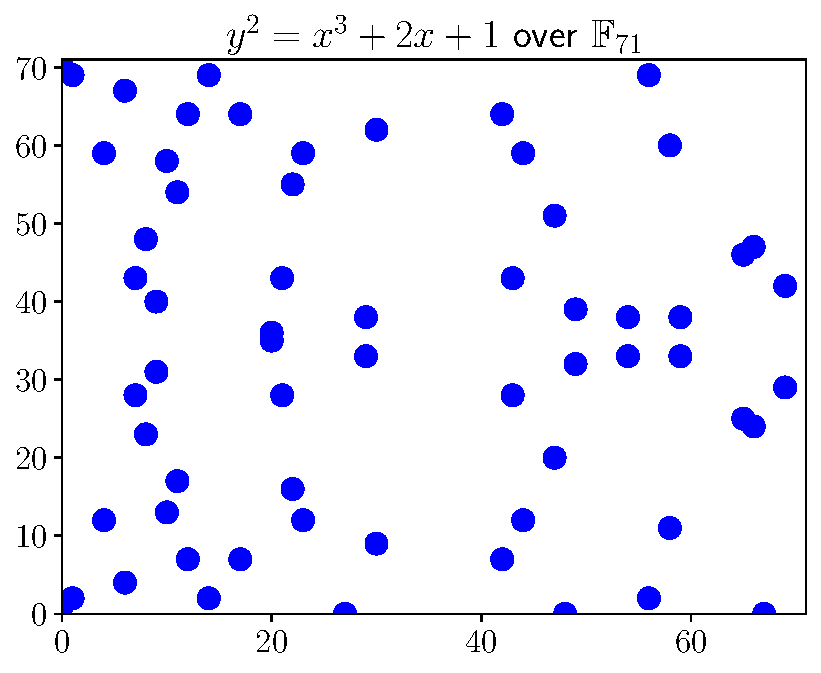
\includegraphics[width=\textwidth]{plots/ec_finite/ec_finite_F_71_2_1_addition_base.pdf}
    \caption{All points on $y^{2} = x^{3} + 2x + 1$ over $\F_{71}$.}
    \end{subfigure}
    \begin{subfigure}[t]{0.45\textwidth}
    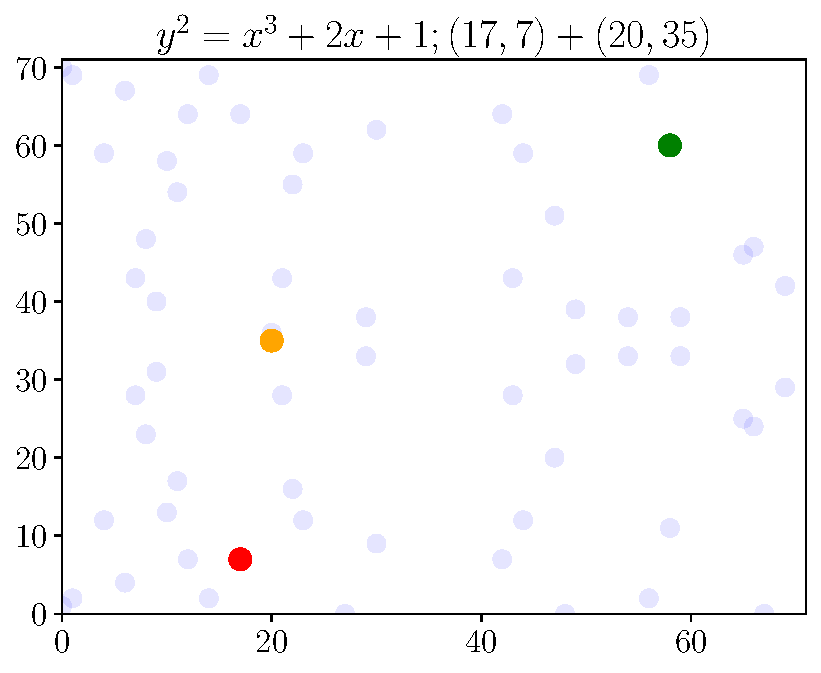
\includegraphics[width=\textwidth]{plots/ec_finite/ec_finite_F_71_2_1_addition_20_35.pdf}
    \caption{$\textcolor{red}{\parens{17,7}}
        + \textcolor{orange}{\parens{20,35}}
        = \textcolor[rgb]{0,0.33,0}{\parens{58,60}}$}
    \end{subfigure}

    \begin{subfigure}[t]{0.45\textwidth}
    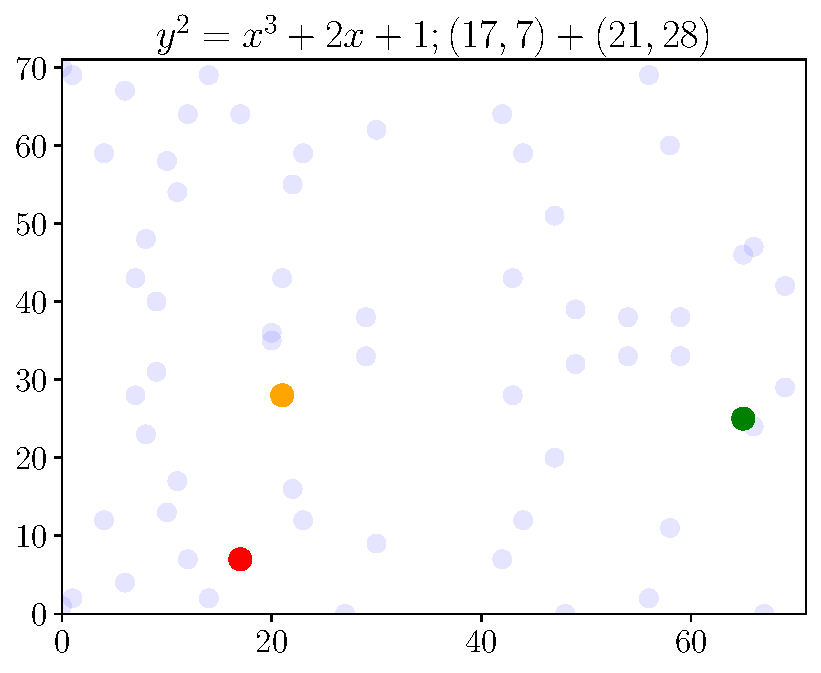
\includegraphics[width=\textwidth]{plots/ec_finite/ec_finite_F_71_2_1_addition_21_28.pdf}
    \caption{$\textcolor{red}{\parens{17,7}}
        + \textcolor{orange}{\parens{21,28}}
        = \textcolor[rgb]{0,0.33,0}{\parens{65,25}}$}
    \end{subfigure}
    \begin{subfigure}[t]{0.45\textwidth}
    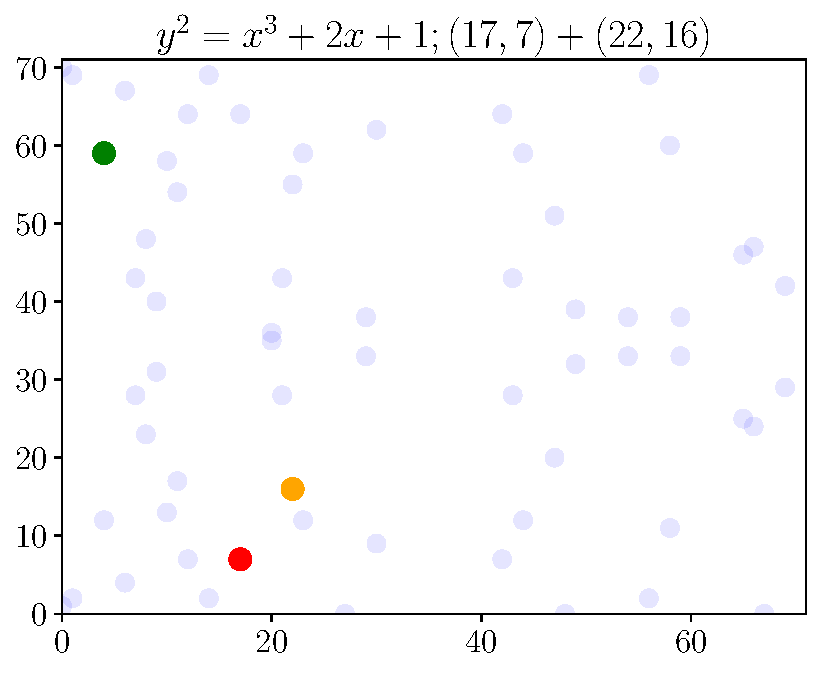
\includegraphics[width=\textwidth]{plots/ec_finite/ec_finite_F_71_2_1_addition_22_16.pdf}
    \caption{$\textcolor{red}{\parens{17,7}}
        + \textcolor{orange}{\parens{22,16}}
        = \textcolor[rgb]{0,0.33,0}{\parens{4,59}}$}
    \end{subfigure}

    \begin{subfigure}[t]{0.45\textwidth}
    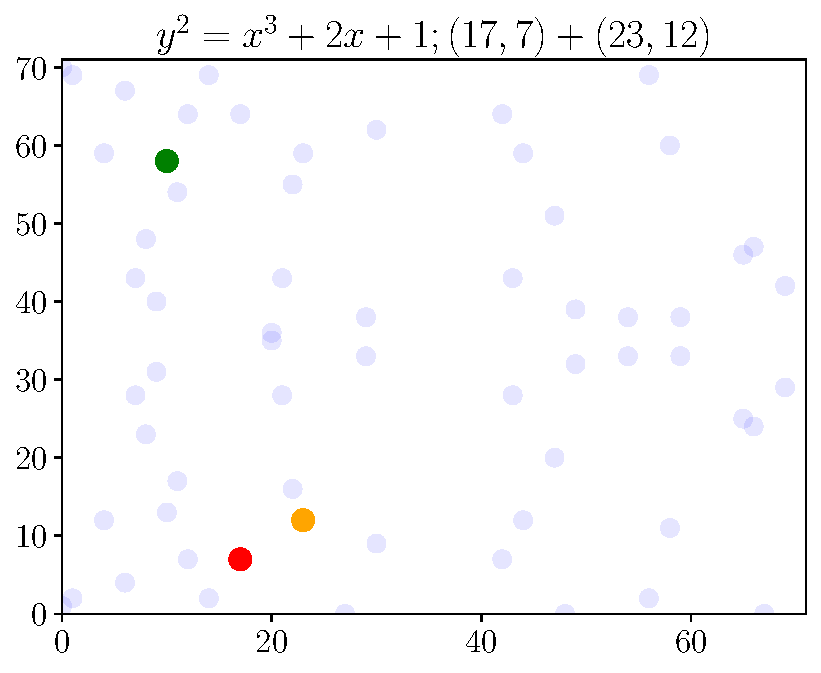
\includegraphics[width=\textwidth]{plots/ec_finite/ec_finite_F_71_2_1_addition_23_12.pdf}
    \caption{$\textcolor{red}{\parens{17,7}}
        + \textcolor{orange}{\parens{23,12}}
        = \textcolor[rgb]{0,0.33,0}{\parens{10,58}}$}
    \end{subfigure}
    \begin{subfigure}[t]{0.45\textwidth}
    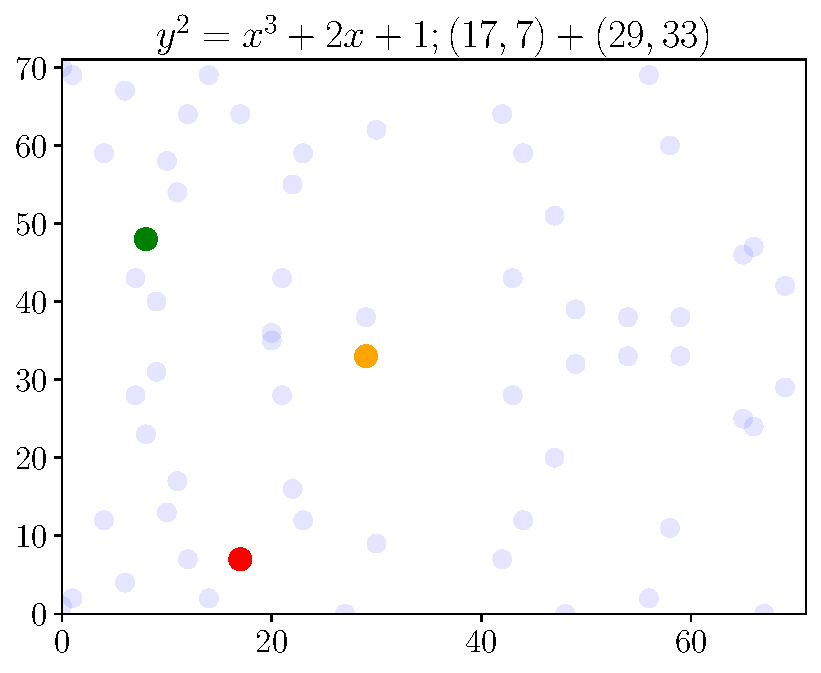
\includegraphics[width=\textwidth]{plots/ec_finite/ec_finite_F_71_2_1_addition_29_33.pdf}
    \caption{$\textcolor{red}{\parens{17,7}}
        + \textcolor{orange}{\parens{29,33}}
        = \textcolor[rgb]{0,0.33,0}{\parens{8,48}}$}
    \end{subfigure}
    \caption[Plots of elliptic curve addition over finite fields]{Here
        have plots of addition on \glspl{elliptic curve} over $\F_{71}$.
        The \glspl{elliptic curve} are all the same: $y^{2} = x^{3} + 2x + 1$.
        The first plot shows the points on the \gls{elliptic curve};
        the other plots show the addition
        $\textcolor{red}{P} + \textcolor{orange}{Q}
            = \textcolor[rgb]{0,0.33,0}{R}$.
        Throughout the plots, $\color{red} P = \parens{17,7}$.
        }
    \label{fig:ec_finite_plots_addition}
\end{figure}
